\documentclass[14pt]{matmex-diploma-custom}

\usepackage{syntax}
\usepackage{listings}
\usepackage[section]{placeins}
\usepackage{float}
\usepackage{graphicx}
\usepackage{amsmath}
\graphicspath{ {./images/} }

\begin{document}
% Год, город, название университета и факультета предопределены,
% но можно и поменять.
% Если англоязычная титульная страница не нужна, то ее можно просто удалить.
\filltitle{ru}{
    chair              = {Факультет Прикадной Математики - Процессов Управления\\ Кафедра технологии программирования},
    title              = {Извлечение данных из учебного контента},
    % Здесь указывается тип работы. Возможные значения:
    %   coursework - Курсовая работа
    %   diploma - Диплом специалиста
    %   master - Диплом магистра
    %   bachelor - Диплом бакалавра
    type               = {bachelor},
    position           = {студента},
    group              = 407,
    author             = {Буланина Екатерина Дмитриевна},
    supervisorPosition = {к.\,ф.-м.\,н., доцент},
    supervisor         = {Добрынин В.\,Ю.},
    reviewerPosition   = {разработчик ЗАО «БИОКАД»},
    reviewer           = {Чуриков Н.\,С.},
    chairHeadPosition  = {к.\,т.\,н., доцент},
    chairHead          = {Блеканов И.\,С.},
%   university         = {Санкт-Петербургский Государственный Университет},
%   faculty            = {Математико-механический факультет},
%   city               = {Санкт-Петербург},
%   year               = {2013}
}
\filltitle{en}{
    chair              = {Applied Mathematics and Control Processes Faculty \\ Programming Technology Chair},
    title              = {Educational data mining},
    author             = {Ekaterina Bulanina},
    supervisorPosition = {},
    supervisor         = {Vladimir Dobrynin},
    reviewerPosition   = {},
    reviewer           = {Nikita Churikov},
    chairHeadPosition  = {},
    chairHead          = {Ivan Blekanov},
}
\maketitle
\tableofcontents
% У введения нет номера главы
\section*{Введение}
За последние десятилетия электронная промышленность достигла колоссальных масштабов, а компьютеры и информационные технологии повсеместно вошли в быт людей. Человечество использует компьютеры для автоматизации всех сфер деятельности: производство и сельское хозяйство, логистика и транспорт, биология и медицина, а также образование.

Если говорить об образовании, то в настоящее время существует множество систем управления обучением (Learning Management System), одним из примеров которых в частности является известный каждому студенту нашего университета BlackBoard~\cite{blackboard}. Такие системы управления образованием предоставляют своим ученикам возможность удалённого обучения онлайн и контроля своих знаний при помощи интерактивных заданий. 

LMS отслеживают различную информацию о своих пользователях:  расписание и список курсов, которые посещает студент; оценки и баллы, полученные в результате выполнения электронных заданий. Всё это --- колоссальные объемы данных, которые потенциально можно использовать для улучшения образовательного процесса. Образовательные данные зачастую детализированны и точны, а их объем очень велик. Анализ данных в сфере образования включает в себя исследования, методы и инструменты, предназначенные для автоматического извлечения данных, связанных с учебной деятельностью людей и создаваемых в образовательных учреждениях.

К примеру, анализ данных в LMS может выявить связь между этапами обучения, к которым студент получил доступ в течение курса, и их итоговой оценкой курса. Аналогично, анализ данных стенограммы студента может выявить связь между оценкой студента по какому-то курсу и его решением изменить свою специализацию. Такая информация дает представление о процессе обучения, что позволяет учащимся и учителям принимать обоснованные решения о том, как взаимодействовать, предоставлять и управлять образовательными ресурсами.

\section{Постановка задачи}
Целью данной работы является автоматическая разметка существующего текстового учебного материала для его дальнейшего переиспользования.

Для достижения этой цели были поставлены следующие задачи: 

\begin{enumerate}
    \item Провести анализ данных, предоставленных ООО <<ИнтеллиДжей Лабс>>~\cite{jetbrains}
    \item Реализовать алгоритм автоматического построения графа тем по учебному контенту~\cite{themegraph}:
    \begin{itemize}
        \item Используя тексты заданий и решения пользователей, привязать задачи к темам в графе
        \item Если какие-то данные остались не размечены, то расширить граф новыми темами % темами или дугами? или и тем и другим? плохо помню суть
    \end{itemize}
\end{enumerate}

\section{Обзор}

\subsection{Терминология}
В качестве основного источника для изучения методов машинного обучения и анализа данных я использовала книгу К. Маннинга <<Введение в информационный поиск>>~\cite{manning}. В этом учебнике рассматривается современный подход ко всем аспектам проектирования и внедрения систем сбора, индексирования и поиска документов, методы оценки систем и использование методов машинного обучения в наборах текстов. В частности, в этой книге описываются алгоритмы стемминга и лемматизации, которые используются в данной работе.

Для ознакомления с областью применения методов машинного обучения и интеллектуального анализа данных в образовательной сфере была использована книга <<Handbook of Educational Data Mining>>~\cite{handbook}. Данная книга содержит исчерпывающий обзор основных методов анализа образовательных данных, а также более двадцати реальных случаев применения этих методов на практике.
\subsection{Литература}
В большинстве случаев знания студентов оцениваются в соответствии с какой-то измерительной шкалой, например от 2 до 5 баллов за экзамен или от 0 до 100 баллов за тест. Авторы работы <<Knowledge Spaces and Learning Spaces>>~\cite{knowspaces} дают представление о том, как дать оценку умениям и навыкам студентов иным образом. Основная идея заключается в том, чтобы воспринимать полученные человеком знания как набор освоенных им <<концепций>>, принимая при этом во внимание предыдущие результаты. Знания при этом представляются нелинейно в виде графа, в котором эти темы или концепции расположены с учётом трудности их понимания и взаимосвязи друг с другом. Так, в вершинах графа находятся концепции, а ребра графа показывают порядок их изучения. Работа представляет большой интерес, потому что в ней формально описываются способы оценки полученных знаний при помощи распределения вероятностей правильных ответов на тестовые вопросы. Подобная методика могла быть использована в адаптивных онлайн-курсах, один из которых используется в моей работе.

Вдохновляющим примером разметки учебного материала послужила статья <<Toward the Automatic Labeling of Course Questions for
Ensuring their Alignment with Learning Outcomes>>~\cite{paper44}, опубликованная в 2017 году на конференции, посвященной анализу данных в сфере образования. В статье была рассмотрена задача классификации экзаменационных вопросов в соответствии с таксономией Блума~\cite{bloom}. Данная работа интересна тем, что решает задачу разметки контента при помощи метода векторизации TF-IDF, который также будет применяться в ходе моей работы.

В работе <<An Automatic Knowledge Graph Creation Framework from
Natural Language Text>>~\cite{autograph} описывается универсальный подход для расширения графа тем по произвольному тексту на естественном языке. Для этого из текста извлекаются <<тройки>>, элементы которых представляют из себя два объекта и отношение между ними. Затем авторами работы презентуется векторная метрика оценивания схожести таких <<троек>>. Расширения графа новыми темами осуществляется с помощью алгоритма кластеризации таких троек и определения степени соответствия их какому-либо существующему элементу графа.

\section{Архитектура}

Работа над задачей была организована согласно принципам методологии CRISP-DM (CRoss Industry Standard Process for Data Mining)~\cite{crispdm} и представляла из себя три этапа: сбор и исследование данных, подготовка данных и моделирование. Моделирование включает в себя построение модели машинного обучения для привязки задач к темам и создание графа тем по результатам.

Для реализации поставленной задачи использовался язык программирования Python и библиотека алгоритмов машинного обучения Scikit-Learn~\cite{sklearn}, а также язык описания графов DOT~\cite{dot}.

Исходный код разделён на три независимых части: обработка данных, моделирование и построение графа. Обработка данных происходит в два этапа: приведение к единому виду и экстракция необходимых для моделирования данных, затем подготовка данных. Для моделирования использовалось несколько алгоритма машинного обучения для сравнения полученных результатов и определения наиболее точного метода.

<тут картинка>

\section{Реализация}
\subsection{Извлечение и обработка данных}
\subsubsection{Формат данных}
Каждый курс на платформе Stepik состоит из \textit{степов} --- шагов, которые могут представлять из себя просмотр видеоматериалов, решение проверочных заданий или работу с текстом. \textit{Адаптивные} курсы подбирают задания индивидуально для каждого пользователя платформы, основываясь на уровне знаний, личной оценке той или иной задачи пользователем, а также затраченном времени. Курс <<Adaptive Python>>~\cite{adapython}, для которого необходимо построить граф тем, представляет из себя адаптивный тренажёр для обучению языку программирования Python~\cite{Python}. 

Для извлечения необходимых данных курса <<Adaptive Python>> было использовано Stepik REST API~\footnote{REpresentational State Transfer Application Programming Interface} --- программный интерфейс платформы Stepik, позволяющий автоматически обращаться к её ресурсам. Компанией JetBrains были предоставлены данные о степах и попытках (как удачных, так и неудачных) решения задач этих степов пользователями платформы.

В предоставленном наборе данных каждому степу соответствовал набор \textit{тем} --- некоторых <<тэгов>>, описывающих содержательную часть задания (к примеру, <<Целые числа>> или <<ООП>>). Помимо этого, для каждой темы был указан её идентификатор в базе знаний <<Wikidata>>~\cite{wikidata}. В данных о попытках решения для каждого степа помимо кода решения на языке Python было также указано, являлось ли решение верным. Данные были представлены в формате рабочей книги Microsoft Excel (.xlsx)~\footnote{формат данных программы для работы с электронными таблицами} и текстовом формате представления таблицы Comma-Separated Values (.csv)~\footnote{значения колонок таблицы разделены запятой}. Для обработки этих форматов были использованы библиотеки openpyxl~\cite{openpyxl} и pandas~\cite{pandas}.

\subsubsection{Извлечение данных}
Полученные данные содержали несущественные для решения поставленной задачи значения и были представлены в разных форматах, поэтому для удобства было принято решение в дальнейшем использовать формат представления JSON~\footnote{JavaScript Object Notation --- основанный на языке программирования JavaScript формат обмена данными, преимуществом которого является удобство чтения как человеком, так и компьютером}.

Формулировки заданий курса было решено исключить из рассмотрения, поскольку они зачастую слишком абстрактны и от студента курса требуется самостоятельно составить требования к решению. Более полезным для привязки того или иного степа курса к набору тем будет анализ кода решения, полученного платформой от пользователем. Поэтому из предоставленных данных были извлечены попытки решения пользователей того или иного задания, а также существующий список тем, соответствующих заданию.

\subsubsection{Предобработка}
Решения пользователей представляют из себя тексты кода на языке Python. Для построения модели было решено взять только верные попытки решения задач. Коды этих попыток были протестированы внутренней системой Stepik и удовлетворяют условиям заданий. К тому же, среди неверных попыток оказывается слишком много пустых или синтаксически некорректных блоков кода.

Поскольку степы адаптивного курса представляют из себя классические задачи по программированию, коды правильных решений в большинстве своём по структуре оказываются очень похожи. Однако они всё же отличаются названиями переменных, а также наличием или отсутствием в них комментариев, которые могут быть самыми разнообразными. В ходе экспериментов было обнаружено, что различное именование переменных отрицательно влияет на результат моделирования: одну и ту же целочисленную переменную-счетчик разные студенты могут назвать $x$, $a$, $i$, $k$, $n$; переменную для размера массива называют $size$, $length$, $count$.

Поэтому было принято решение предобработать коды таким образом, чтобы очистить их от комментариев, а также переименовать все переменные единым образом. Процесс предобработки состоит из трех этапов: синтаксический анализ, унификация переменных и pretty-printing.

\subsubsection*{Синтаксический анализ}
На первом этапе для исходного кода строится его синтаксическое дерево с помощью парсера из библиотеки ast~\cite{ast}.

\subsubsection*{Унификация переменных}
Далее для каждого синтаксического дерева запускается процесс унификации переменных. Он состоит из двух рекурсивных обходов дерева, которые представляют из себя реализации стандартного для деревьев шаблона проектирования <<Посетитель>>~\cite{DesignPatterns}. Сначала первый посетитель VariablesCollector обходит дерево, собирает все имена переменных и назначает каждому имени свой номер. Затем второй посетитель VariablesRenamer переименовывает все переменные, назначая им имена $i_1$, $i_2$ и т.д. в соответствии с номером.

\subsubsection*{Pretty-printing}
Pretty-printing~\cite{pretty-printing} --- это форматирование исходного кода в соответствии с некоторым заданным стилем. Модели, использованные в работе, оперируют с текстами, а не деревьями, поэтому по итогу предобработки мы должны снова получить текст программы. Как и в случае с разными названиями переменных, модели показывают худшие результаты на текстах с разными стилями оформления (например, с разной табуляцией, отступами и переносами или отсутствием переносов строк). Поэтому каждое синтаксическое дерево печатается в некотором едином стиле. Эта печать реализуется с помощью pretty-printer --- ещё одного посетителя, который обходит все вершины и печатает текст для каждой из них.

\subsection{Построение модели}
\subsubsection{Входные данные и необходимые метрики}
Для обучение модели классификации по нескольким меткам (Multi-label classification~\footnote{задача классификации, при которой каждому объекту сопоставляется один или несколько классов}) извлечённые данные были разделены на тренировочные и тестовые. Для этого данные были перемешаны с помощью генератора случайных чисел, затем 70\% данных были отмечены как тренировочные, а 30\% будут затем использоваться для проверки обученной модели.

Рассмотрим метрики для определения точности классификации.

\subsubsection*{Accuracy}

Простейшая метрика, представляющая из себя долю верно классифицированных объектов среди всего размера обучающей выборки.
\[
\text{Accuracy}=\frac{\{\text{correct}\}}{\{\text{train sample}\}}
\]

\subsubsection*{Precision and recall}

Точность классификатора определяется как доля верно классифицированных объектов среди всех объектов, отнесённых классификатором к классу k:

\[
\text{Precision}_{k}=\frac{|\{\text{relevant}\}\cap\{\text{retrieved}\}|}{|\{\text{retrieved}\}|}
\]

Точность отвечает на вопрос: сколько из всех выбранных объектов действительно принадлежат классу k?

Полнота определяется как доля верно классифицированных объектов среди всех объектов класса k в тестовой выборке:

\[
\text{Recall}_{k}=\frac{|\{\text{relevant}\}\cap\{\text{retrieved}\}|}{|\{\text{relevant}\}|}
\]

Полнота отвечает на вопрос: сколько из всех действительно принадлежащих классу k объектов были выбраны?

\subsubsection*{F1-score}

F1-мера определяется как среднее гармоническое между точностью и полнотой класса k:

\[
\text{F1-score}_{k}=\frac{2\cdot\text{Precision}_{k}\cdot\text{Recall}_{k}}{\text{Precision}_{k} + \text{Recall}_{k}}
\]

Как видно, F1-мера стремится к нулю, если точность или полнота стремится к нулю. При этом одинаковый вес придаётся обоим этим метрикам.

Общая формула для оценки F$\beta$ -score, которая придаёт больший вес полноте на порядок $\beta$:

\[
\text{F$\beta$}_{k}=\frac{(1+\beta^2)\cdot\text{Precision}_{k}\cdot\text{Recall}_{k}}{\beta^2\cdot\text{Precision}_{k} + \text{Recall}_{k}}
\]

\subsubsection*{Support}

Метрика поддержки показывает для класса k количество объектов, ему принадлежащих. Данное значение служит коэффициентом для вычисления средних значений \text{Precision} и \text{Recall} по всем классам.

\subsubsection{Предсказание тем} 
Для того, чтобы привязать уроки онлайн-курса к темам, используется векторная модель представления их решений. Предсказанные на данном этапе темы впоследствии будут соответствовать некоторому пути в графе тем.

\subsubsection*{TF-IDF представление}

Для векторизации решений заданий курса используется TF-IDF мера. Введем необходимые обозначения и определения:

\begin{itemize}
    \item \textit{Документ} --- текстовые данные, состоящие из набора лексем. В нашем случае документом является текстовое представление решения пользователя.
    \item \textit{TF \text{(term frequency)}} --- отношение числа вхождения определенной лексемы $n_{i}$ к общему количеству лексем в документе:
    \[
    \text{TF}=\frac{n_{i}}{\sum_{k}n_{k}}
    \]
    \item \textit{IDF \text{(inverse document frequency)}} --- обратная документная частота, определяемая следующим образом: 
    \[
    \text{IDF}=\log\frac{N}{df}
    \]
    \\N --- количество документов в коллекции
    \\df --- количество документов, содержащиз $n_{i}$.
    \item \textit{TF-IDF} --- мера, определяющая вес каждой лексемы в каждом документе:
    \[
    \text{TF-IDF}= \text{TF}\cdot\text{IDF}
    \]
    Мера \textit{TF-IDF} уменьшается, когда лексема встречается в большом количестве документов, и увеличивается, если лексема встречается часто в небольшом количестве документов.
\end{itemize}

Задача привязки заданий к темам рассматривается в работе как задача классификации по $k$ категориям. Для этого используются представленные ниже классификаторы, результаты работы которых будут сопоставлены в соответствии с приведенными выше метриками.

\subsubsection*{One vs Rest}

Задача классификации данных (в нашем случае заданий) по $k$ категориям может быть сведена к $k$ задачам бинарной классификации. Для каждого из классов обучается свой классификатор, определяющий принадлежность либо не принадлежность классу. Так работает классификатор One vs Rest. Помимо вычислительной эффективности и простоты имплементации, преимуществом данной классификации является легкость интерпретации полученных данных.

\subsubsection*{$K$ Neighbors}

Алгоритм $k$-ближайших соседей --- простейший алгоритм классификации и регрессии для задач обучения с учителем. Классификатор использует метрику (например, стандартную в евклидовом пространстве) для вычисления расстояния между объектами выборки, и определяет класс каждого из объектов как наиболее часто встречающийся среди $k$ его ближайших по метрике соседей. Несмотря на недостатки алгоритма, например необходимость настройки параметров, было принято решение попробовать его как классический и наиболее простой вариант.

\subsubsection*{Multinomial Naive Bayesian Classifier}
Мультиномиальный наивный байесовский классификатор представляет из себя вероятностную модель с применением теоремы Байеса в предположении о независимости. Классификатор определяет искомый класс объекта как класс, имеющий максимальную \textit{апостериорную} вероятность. Для избежания потери значимых разрядов при умножении зачастую используют сумму логарифмов вероятностей вследствие монотонности логарифмической функции и равенства \log(x\cdot y) = \log(x)+\log(y).

\subsubsection*{Decision Tree}
Алгоритм решающих деревьев --- логический алгоритм классификации, задающийся бинарным деревом, используется во множестве задач регрессии и классификации. Каждому листу дерева соответствует класс, и при классификации того или иного объекта алгоритм проходит весь путь от корня до некоторого листа, определяя тем самым класс. Для построения алгоритма необходимо выбрать признак разделения и минимальный порог (если необходим). 

\subsubsection*{Random Forest}
Случайный лес --- ансамбль решающих деревьев, эффективно используемый для обработки данных с большой размерностью. Основными преимуществами данного метода машинного обучения являются высокая масштабируемость и параллелизуемость. Один из его недостатков --- склонность к переобучению на зашумлённых данных.

\subsection{Построение и расширение графа}
\subsubsection{Обозначения}
Введем необходимые обозначения и определения:

\begin{itemize}
\item $\mathcal{T}$ --- множество всех тем онлайн-курса.
    \item \textit{Урок} (степ) --- множество тем $\{t_i\}$, соответствующее какому-то конкретному занятию онлайн-курса.
    \item $\mathcal{L}$ --- множество всех уроков онлайн-курса.
    \item $\mathcal{G}$ --- направленный граф тем; его вершинами являются элементы множества $\mathcal{T}$, а дуги соответствуют порядку изучения тем 
\end{itemize}

Сначала необходимо получить первое приближение $G_0$ искомого графа $G$. Вершинами обоих графов являются исходные темы онлайн-курса. Для построения дуг используются данные из Wikidata: с помощью запросов на языке SPARQL~\cite{SPARQL} проверяется, как темы соотносятся между собой. Тема $t_1$ считается предком темы $t_2$, если для них имеет место отношение "instance of", "subclass of" или "part of". 

В рамках расширения графа тем предполагается, что каждый урок соответствует некоторому пути в искомом графе, то есть 
$$\forall~ l \in \mathcal{L} ~\exists~ (t_1, t_2, ..., t_n) \in \mathcal{G} : l = \{t_1, t_2, ..., t_n\}$$

Основная идея построения графа состоит в том, чтобы сначала найти топологическую сортировку расширенного графа, а затем по ней построить сам расширенный граф.

Для описания алгоритма нам потребуется ещё несколько вспомогательных обозначений:

$count(t_i) = |\{l \in \mathcal{L} : t_i \in l \}|$ -- количество уроков с этой темой

$preds(t_i) = \{t \in \mathcal{T} : \exists~ (t, ..., t_i) \in \mathcal{G}\}$ -- предки $t_i$ в графе $\mathcal{G}$

$neighbors(t_i)$ -- соседние темы $t_i$ \\ % TODO: что за соседние темы? непонятно

\subsubsection{Алгоритм расширения}

\begin{enumerate}
    \item Составить словарь $\forall~ t_i \in \mathcal{T}~ \{ t_i: count(t_i) \}$
    
    \item В каждом уроке отсортировать темы $t_i$ по убыванию $count(t_i)$
    
    \item Составить словарь $\forall t_i \in \mathcal{T}~ \{ t_i: neighbors(t_i) \}$; в дальнейшем считаем, что $neighbors(t_i)$ являются предками $t_i$
    \item Отсортировать уроки по убыванию количества тем в них
    
    \item Пронумеровать уроки уровнями в соответствии с топологической сортировкой: $\forall t_i \in \mathcal{T}: level[t_i] \in [0..N]$
    
    Теперь мы знаем уровни вершин (т.е. длины путей от одной из корневых вершин).
    Осталось добавить в граф ребра в соответствии с уровнями и уроками (как упоминалось выше, каждый урок соответствует некоторому пути)
    
    \item Проходим по всем уровням от 0 до последнего:
    для каждой темы добавляем ребра из его предков, если тема ещё недостижима из предка.
    
    Достижимость вершины проверяется с помощью поиска в глубину или алгоритма Флойда-Уоршалла.
\end{enumerate}

В результате выполнения алгоритма заданный граф $\mathcal{G_0}$ расширяется новыми дугами. % и темами?

\section{Апробация}

\subsection{Построение графа тем}
Был построен граф тем, каждой из вершин которого соответствует задание курса. Для наглядности исходный граф был значительно сокращён. Полноразмерный вариант графа, а также соответствие заданий и путей в нём, приведены вместе с исходным кодом проекта на ресурсе GitHub~\footnote{\url{https://github.com/shabatar/knowledge-spaces}}.
\begin{figure}[!htb]
\caption{Сокращённый вариант построения графа тем}
\hspace*{-2cm}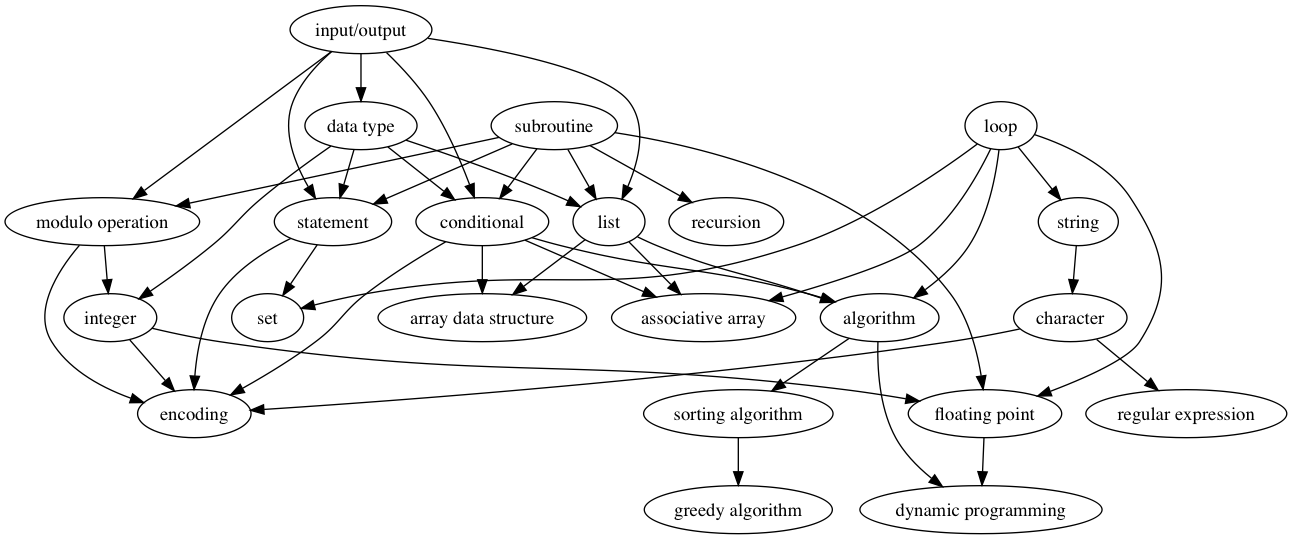
\includegraphics[width=20cm]{themegraph}
\label{themegraph}
\end{figure}

\subsection{Привязка заданий к темам}
В ходе апробации было проведено сравнение нескольких перечисленных методов классификации по темам. Для этого использовалась композиция метрик Precision, Recall и F1-score. Поскольку наилучшим образом справился с задачей метод Decision Tree, ниже на Рис.~\ref{report} приведена таблица значений метрик по каждому из классов, определенных при помощи данного классификатора.

\begin{figure}
\caption{Результат Decision Tree Classifier для данных.}
\center{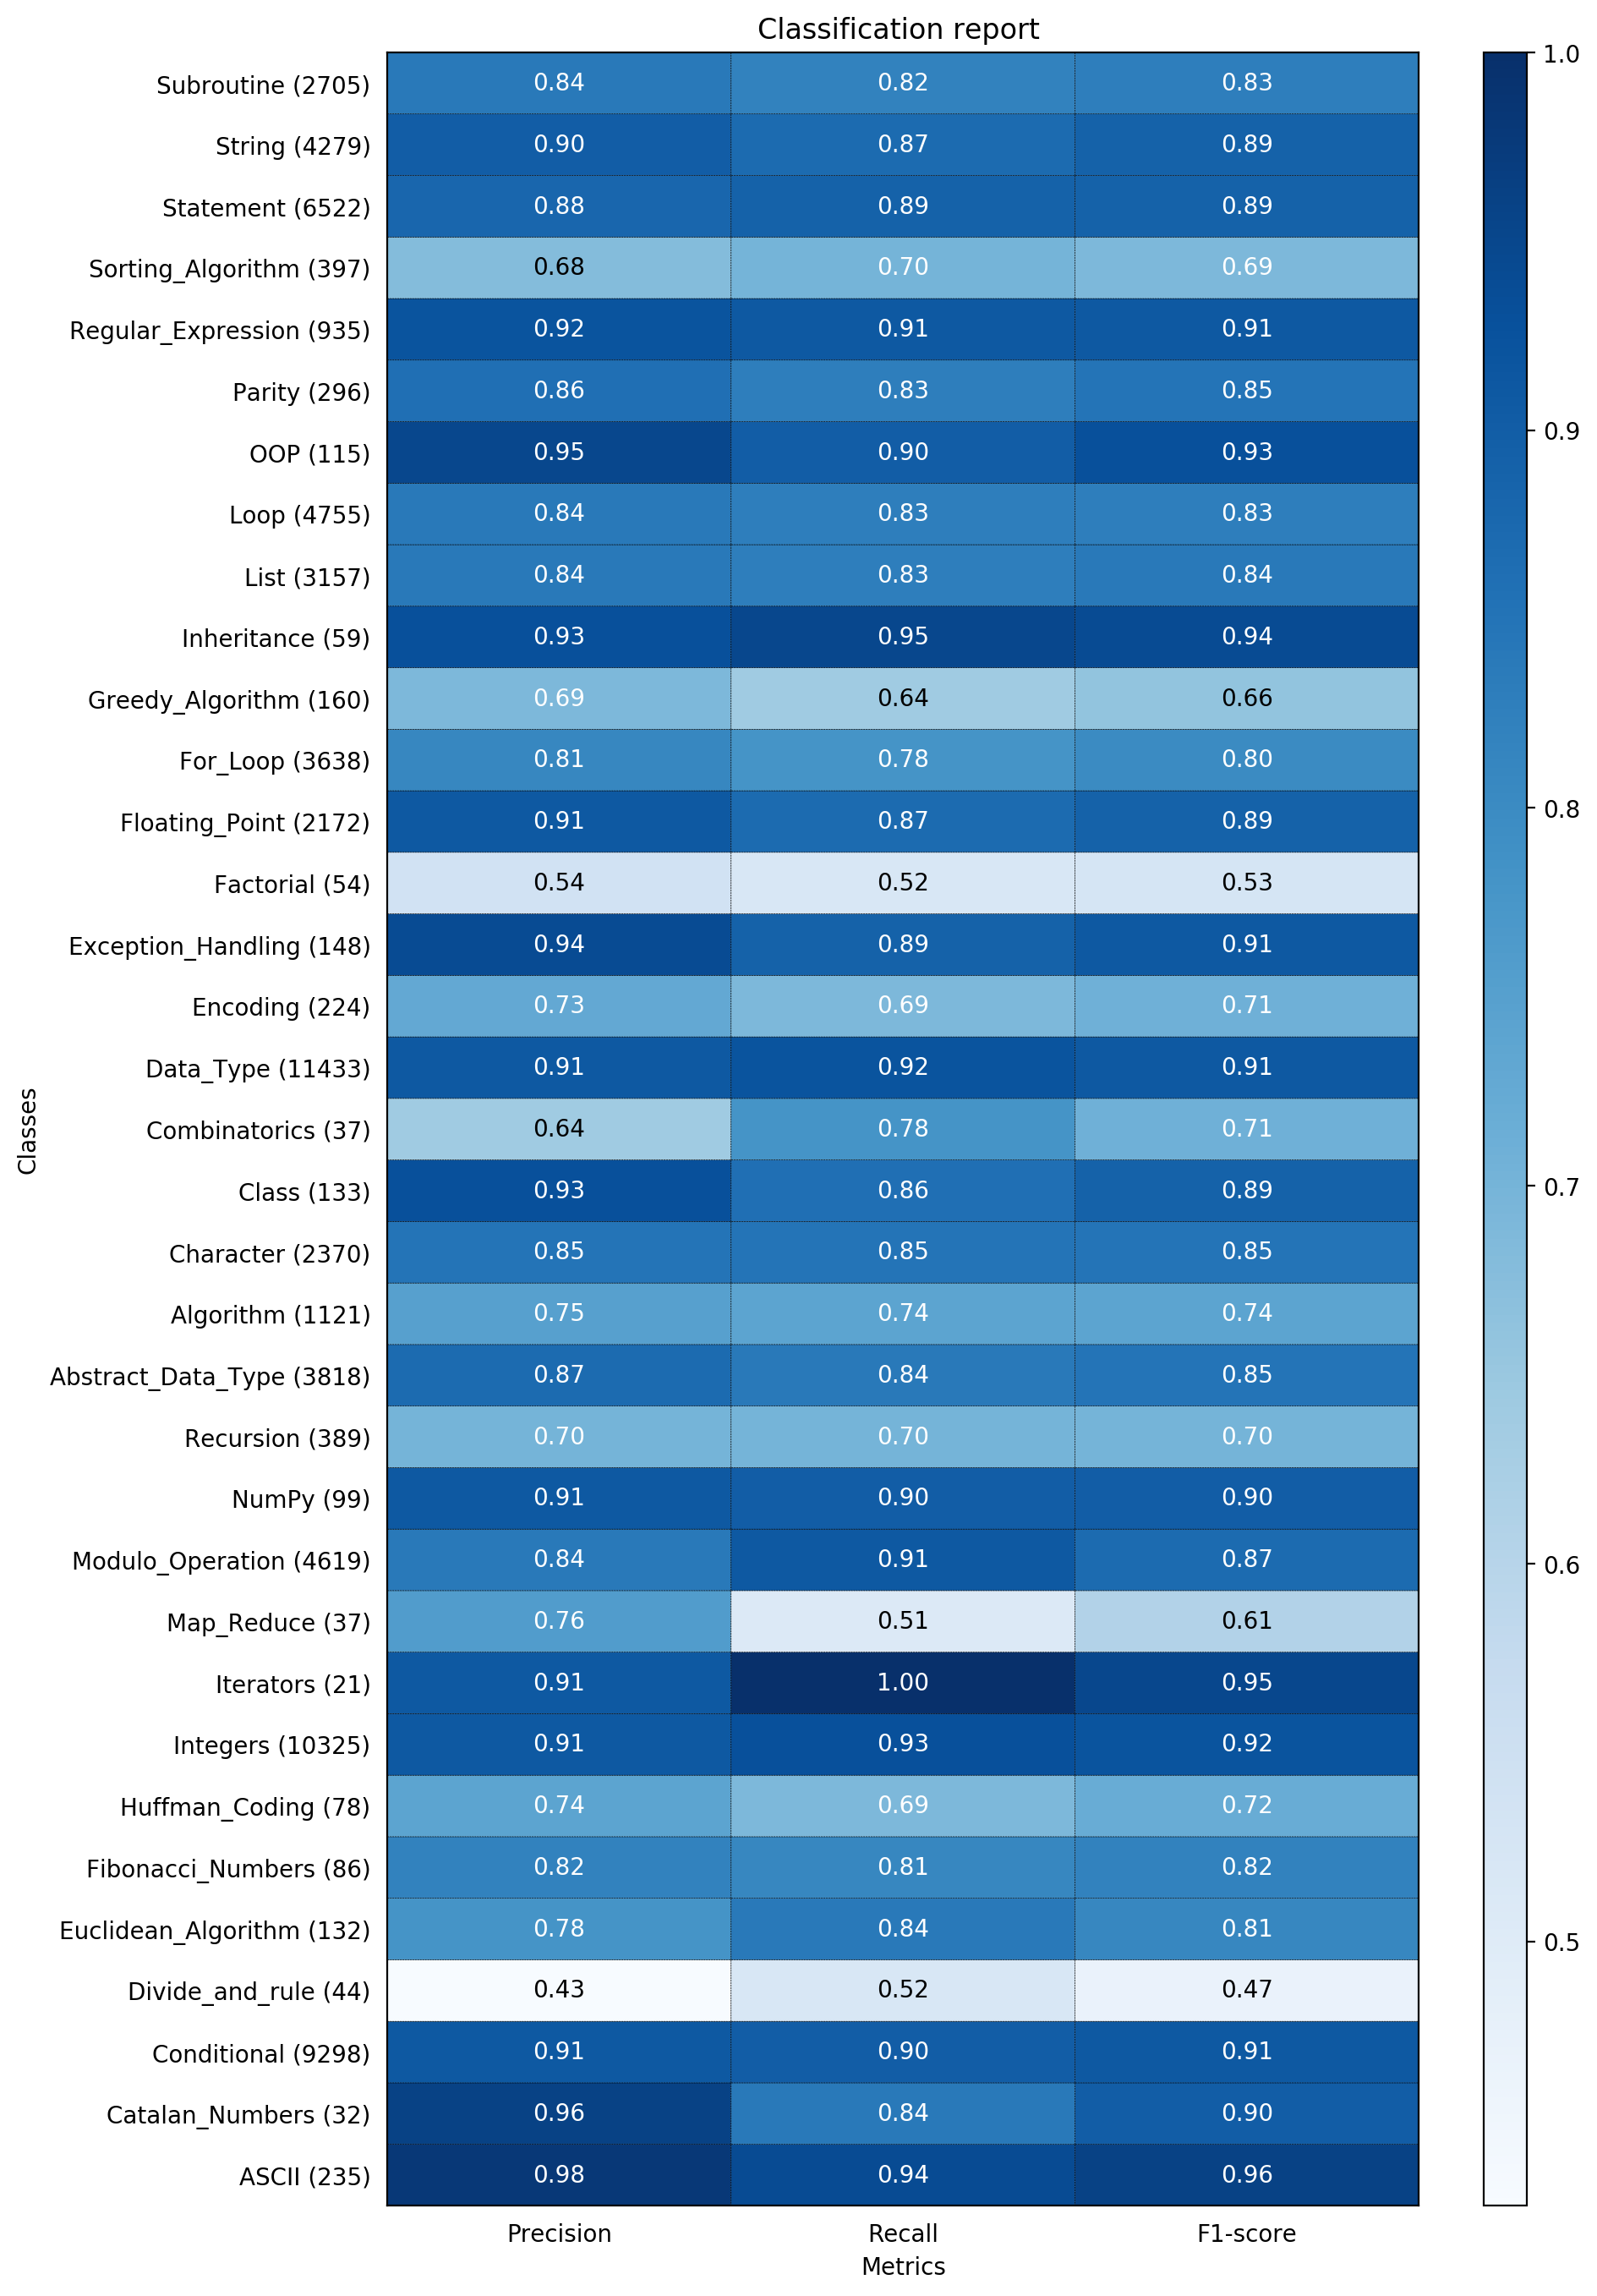
\includegraphics[scale=0.65]{report}}
\label{report}
\end{figure}


% У заключения нет номера главы
\section*{Заключение}
В ходе данной работы были получены следующие результаты:

\begin{enumerate}
    \item Проведён анализ предметной области. Сделан обзор аналогичных существующих решений, используемых в них методов анализа данных и машинного обучения, а также метрик для оценки результатов их работы. 
    \item Реализован алгоритм многоклассовой классификации извлечённых данных. Он затем используется для привязки задач онлайн-курса к той или иной вершине в графе тем. Были протестированы варианты реализации алгоритма с различными классификаторами. В результате наилучшим образом себя показал метод решающего дерева.
    \item Реализован метод автоматического построения графа тем по учебному контенту:
    \begin{itemize}
        \item Используя результаты работы классификатора на предыдущем шаге, задачи курса привязываются к темам в графе.
        \item Используя идею топологической сортировки, реализован алгоритм расширения полученного графа новыми вершинами.
    \end{itemize}
\end{enumerate}

\setmonofont[Mapping=tex-text]{CMU Typewriter Text}
\bibliographystyle{ugost2008ls}
\bibliography{diploma.bib}
\end{document}
